%!TEX TS-program = xelatex
\documentclass[12pt, a4paper, oneside]{article}

\usepackage{amsmath,amsfonts,amssymb,amsthm,mathtools}  % пакеты для математики

\usepackage[english, russian]{babel} % выбор языка для документа
\usepackage[utf8]{inputenc} % задание utf8 кодировки исходного tex файла
\usepackage[X2,T2A]{fontenc}        % кодировка

\usepackage{fontspec}         % пакет для подгрузки шрифтов
\setmainfont{Linux Libertine O}   % задаёт основной шрифт документа

\usepackage{unicode-math}     % пакет для установки математического шрифта
\setmathfont[math-style=upright]{Neo Euler} % шрифт для математики

% Конкретный символ из конкретного шрифта
% \setmathfont[range=\int]{Neo Euler}

%%%%%%%%%% Работа с картинками %%%%%%%%%
\usepackage{graphicx}                  % Для вставки рисунков
\usepackage{graphics}
\graphicspath{{images/}{pictures/}}    % можно указать папки с картинками
\usepackage{wrapfig}                   % Обтекание рисунков и таблиц текстом

%%%%%%%%%%%%%%%%%%%%%%%% Графики и рисование %%%%%%%%%%%%%%%%%%%%%%%%%%%%%%%%%
\usepackage{tikz, pgfplots}  % язык для рисования графики из latex'a

%%%%%%%%%% Гиперссылки %%%%%%%%%%
\usepackage{xcolor}              % разные цвета

\usepackage{hyperref}
\hypersetup{
	unicode=true,           % позволяет использовать юникодные символы
	colorlinks=true,       	% true - цветные ссылки, false - ссылки в рамках
	urlcolor=blue,          % цвет ссылки на url
	linkcolor=red,          % внутренние ссылки
	citecolor=green,        % на библиографию
	pdfnewwindow=true,      % при щелчке в pdf на ссылку откроется новый pdf
	breaklinks              % если ссылка не умещается в одну строку, разбивать ли ее на две части?
}


\usepackage{todonotes} % для вставки в документ заметок о том, что осталось сделать
% \todo{Здесь надо коэффициенты исправить}
% \missingfigure{Здесь будет Последний день Помпеи}
% \listoftodos --- печатает все поставленные \todo'шки

\usepackage[paper=a4paper, top=20mm, bottom=15mm,left=20mm,right=15mm]{geometry}
\usepackage{indentfirst}       % установка отступа в первом абзаце главы

\usepackage{setspace}
\setstretch{1.15}  % Межстрочный интервал
\setlength{\parskip}{4mm}   % Расстояние между абзацами
% Разные длины в латехе https://en.wikibooks.org/wiki/LaTeX/Lengths


\usepackage{xcolor} % Enabling mixing colors and color's call by 'svgnames'

\definecolor{MyColor1}{rgb}{0.2,0.4,0.6} %mix personal color
\newcommand{\textb}{\color{Black} \usefont{OT1}{lmss}{m}{n}}
\newcommand{\blue}{\color{MyColor1} \usefont{OT1}{lmss}{m}{n}}
\newcommand{\blueb}{\color{MyColor1} \usefont{OT1}{lmss}{b}{n}}
\newcommand{\red}{\color{LightCoral} \usefont{OT1}{lmss}{m}{n}}
\newcommand{\green}{\color{Turquoise} \usefont{OT1}{lmss}{m}{n}}

\usepackage{titlesec}
\usepackage{sectsty}
%%%%%%%%%%%%%%%%%%%%%%%%
%set section/subsections HEADINGS font and color
\sectionfont{\color{MyColor1}}  % sets colour of sections
\subsectionfont{\color{MyColor1}}  % sets colour of sections

%set section enumerator to arabic number (see footnotes markings alternatives)
\renewcommand\thesection{\arabic{section}.} %define sections numbering
\renewcommand\thesubsection{\thesection\arabic{subsection}} %subsec.num.

%define new section style
\newcommand{\mysection}{
	\titleformat{\section} [runin] {\usefont{OT1}{lmss}{b}{n}\color{MyColor1}} 
	{\thesection} {3pt} {} } 


%	CAPTIONS
\usepackage{caption}
\usepackage{subcaption}
%%%%%%%%%%%%%%%%%%%%%%%%
\captionsetup[figure]{labelfont={color=Turquoise}}

\pagestyle{empty}

%%%%%%%%%% Свои команды %%%%%%%%%%
\usepackage{etoolbox}    % логические операторы для своих макросов

% Все свои команды лучше всего определять не по ходу текста, как это сделано в этом документе, а в преамбуле!

% Одно из применений - уничтожение какого-то куска текста!
\newbool{answers}
%\booltrue{answers}
\boolfalse{answers}

\usepackage{enumitem}
% бульпоинты в списках
\definecolor{myblue}{rgb}{0, 0.45, 0.70}
\newcommand*{\MyPoint}{\tikz \draw [baseline, fill=myblue,draw=blue] circle (2.5pt);}
\renewcommand{\labelitemi}{\MyPoint}

% расстояние в списках
\setlist[itemize]{parsep=0.4em,itemsep=0em,topsep=0ex}
\setlist[enumerate]{parsep=0.4em,itemsep=0em,topsep=0ex}


\begin{document}
	
\section*{Семинар 6: Регрессия}

В этом семинаре мы впервые столкнёмся с настоящим машинным обучением и попробуем понять что стоит за его магией. В ручной части семинара мы пойдём по следующему  плану: 

\begin{itemize}
	\item разберёмся чем классификация отличается от регрессии ;
	\item сформулируем задачу регрессии и поймём её специфику;
	\item поймём с помощью каких метрик можно оценить качество прогноза в случае регрессии;
	\item попробуем разобраться какой смысл стоит за этими метриками;
	\item разберёмся как выглядит простейшая линейная модель регрессии;
	\item на пальцах прикинем как она обучается.
\end{itemize}


\subsection*{Задача 1 (формулируем задачу)}

Представьте себе, что у вас есть паблик с мемами. Вы --- Хозяин мемов. Как и любой другой Хозяин мемов, вы любите лайки под мемами. Возникает желание привлечь в паблик целевую аудиторию, которая будет ставить под мемы лайки. Для этого вы хотите запустить рекламную кампанию паблика. Ясное дело, что рекламу хочется показывать не всем подряд,  а только подходящим людям. 

У вас есть данные по профилям всех тех людей, которые уже ставили в паблике лайки. По этим данным вам хочется построить модель, котороя могла бы предсказать подходит ли конкретный человек для вашей рекламной компании (поставил бы ли он в паблик лайк, если бы был на него подписан). 

\begin{enumerate}
\item Сформулируйте задачу машинного обучения. Какой должна быть целевая переменная, чтобы перед вами была задача классификации. Какой должна быть целевая переменная, чтобы это была задача регрессии? 

\item Какие факторы из профилей вы бы использовали, чтобы спрогнозировать подходит ли человек для рекламной кампании?

\item Приведите ещё парочку примеров задачи классификации и задачи регрессии. 
\end{enumerate}

\ifbool{answers}{
\textbf{Решение:} 

Если мы будем пытаться спрогнозировать факт лайка (пользователь поставил хотя бы один лайк в паблик), то мы будем решать задачу классификации, так как мы стараемся предсказать бинарную переменную. Если мы будем пытаться спрогнозировать непрерывную переменную: количество лайков, которое пользователь поставил в паблике, то мы будем решать задачу регрессии. 

В качестве факторов для прогноза можно использовать абсолютно любую информацию из профилей: пол, возраст, есть ли аватар, как часто человек что-то репостит, на какие другие похожие паблики он подписан и т.п.  Правда не факт, что все эти переменные окажутся полезными. 

\textbf{Классификация:} предсказание оттока клиентов, вернёт ли человек кредит, болен ли человек, содержит ли письмо спам, мошенническая ли транзакция,  сделает ли человек клик,  поставит ли лайк и т.д.

 \textbf{Регрессия:} предсказание цен, спроса, выручки, валютного курса,  ВВП страны, инфляции, качества вина, уровня преступности и т.д.
}

\subsection*{Задача 2 (качество прогноза)}

Добрыня, Алёша и Илья смотрят мемы и ставят на них лайки. Мы пытаемся предсказать сколько лайков они оставят под мемами на основе поведения их однокурсников. Для этого мы оценили регрессию. Ну и она нам напредсказывала, что парни поставят $4$, $20$ и $110$ лайков. В реальности они поставили $5$, $10$ и $100$ лайков. Возникает вопрос: насколько сильно наша модель ошиблась в прогнозировании. Для того, чтобы выяснить это используют различные метрики. Давайте посмотрим на основные. 

Что такое $MAE$, $MSE$, $RMSE$ и $MAPE$?  Посчитайте для модели все четыре метрики качества.

\ifbool{answers}{
	\textbf{Решение:}
	
\begin{itemize}
	
	\item \textbf{MAE (mean absolute error), средняя абсолютная ошибка}
	
	Первой очевидной метрикой качества будет просто взять и просуммировать все ошибки модели. Так, в случае Добрыни ошибка оказалась $|5 - 4| = |1| = 1$. Модуль от ошибки берётся, потому что можно ошибаться в разные стороны. Например, если бы не было модуля, для Алёши ошибка составила бы $10 - 20 = -10$. Потом нам надо было бы сложить две ошибки и мы получили бы $9$. Ошибка в $9$ лайков. А это неправда, потому что мы ошиблись в $11$ лайков. Поэтому берётся модуль. 
	
	Средняя абсолютная ошибка для парней составит: 
	
	$$ 
	\frac{1}{3} \cdot (|5 - 4| + |10 - 20| + |100 - 110|) = 7
	$$
	
	В среднем мы ошибаемся на $7$ лайков. Формула для поиска средней абсолютной ошибки в общем виде выглядит вот так: 
	
	$$ MAE = \frac{1}{n}\sum_{i=1}^{n} |y_i - \hat{y}_i|. $$
	 
	 Можно нарисовать $MAE$ на картинке. По оси $x$ отложим ошибку прогноза. В случае Добрыни это $5-4 = 1$. По оси $y$ будем откладывать то, насколько сильный штраф мы накладываем за такую ошибку. В случае $MAE$ штраф за ошибку в $1$ равен $1$. То есть мы получаем прямую под углом в $45$ градусов. В отрицательную сторону ошибка также штрафуется один к одному. График выглядит как галочка. 
	 	
\begin{center}
	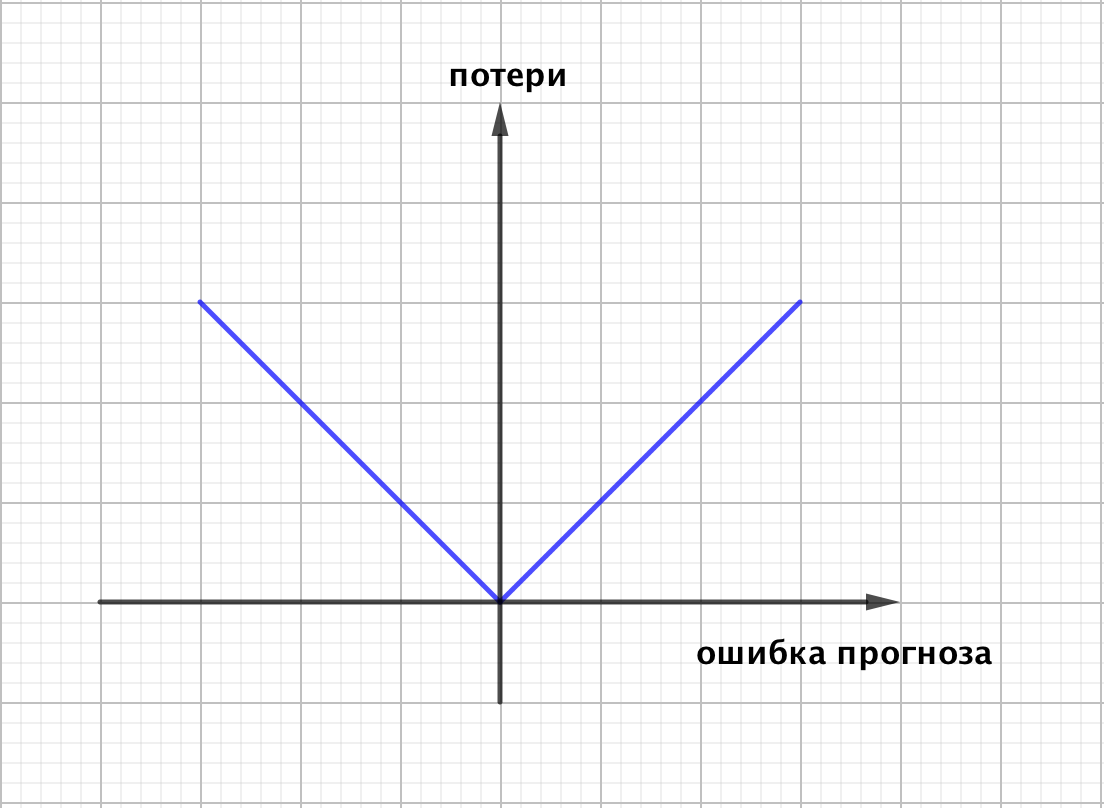
\includegraphics[scale=0.2]{err_mae.png}
\end{center} 	

\item \textbf{квантильная ошибка}

Один из минусов MAE в том, что мы одинаково нелюбим перепрогноз и недопрогноз. В реальности цена этих двух ошибок может быть разной. И мы можем это учесть. Представим себе ситуацию, что хозяин мемов очень сильно обижается, если мы прогнозируем ему больше лайков, чем получается в реальности. Если мы прогнозируем меньше, чем в реальности, он также ошибается, но чуть-чуть. В общем, когда мы делаем перепрогноз, он ошибается в $2$ раза сильнее. Тогда ошибку можно посчитать по формуле: 

$$ 
\frac{1}{3} \cdot (|5 - 4| + 2 \cdot |10 - 20| + 2 \cdot |100 - 110|) = 13.6 
$$

То есть мы умножили перепрогнозы на два. На самом деле в реальности коэффициенты могут быть и другими. Чаще всего они берутся из всяких денежных соображений. В случае, если бы мы прогнозировали не лайки, а продажи в магазине, недопрогноз спроса мог бы для нас быть серьёзнее из-за потери кучи денег в виде лояльных клиентов. Насколько он страшнее мы могли бы попытаться померить в деньгах. Такая неравномерная ошибка обычно называется \textbf{квантильной ошибкой.}

Если мы решим нарисовать такую ошибку на картинке, наша галочка чуть-чуть покорёжится. 
	
\begin{center}
	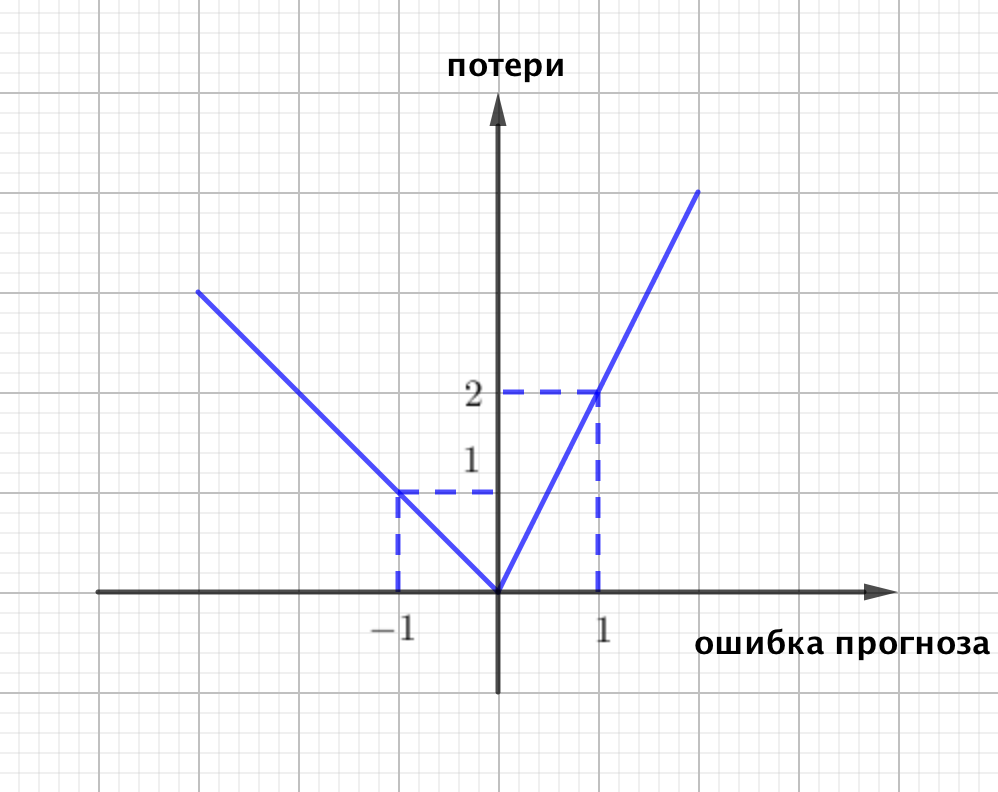
\includegraphics[scale=0.2]{err_quan.png}
\end{center} 	

Увидели? Теперь, если мы ошибаемся на единицу направо, то есть происходит перепрогноз, мы несём потери размером $2$. Если мы ошибаемся налево на единицу, то есть происходит недорогноз, мы несём потери в $1$. Получается, что любой сдвиг вправо в плане ошибки для нас в два раза хуже, чем влево.  Чем больше коэффициент перед ошибкой, тем резче дисбаланс в ошибках для нас. 

\item \textbf{Кусочно-линейная функция потерь} 
	
Можно немного модернизировать квантильную ошибку и преварить её в кусочно-линейную функцию потерь. Такая функция неплохо подойдёт для задачи прогнозирования продаж. 

\begin{center}
	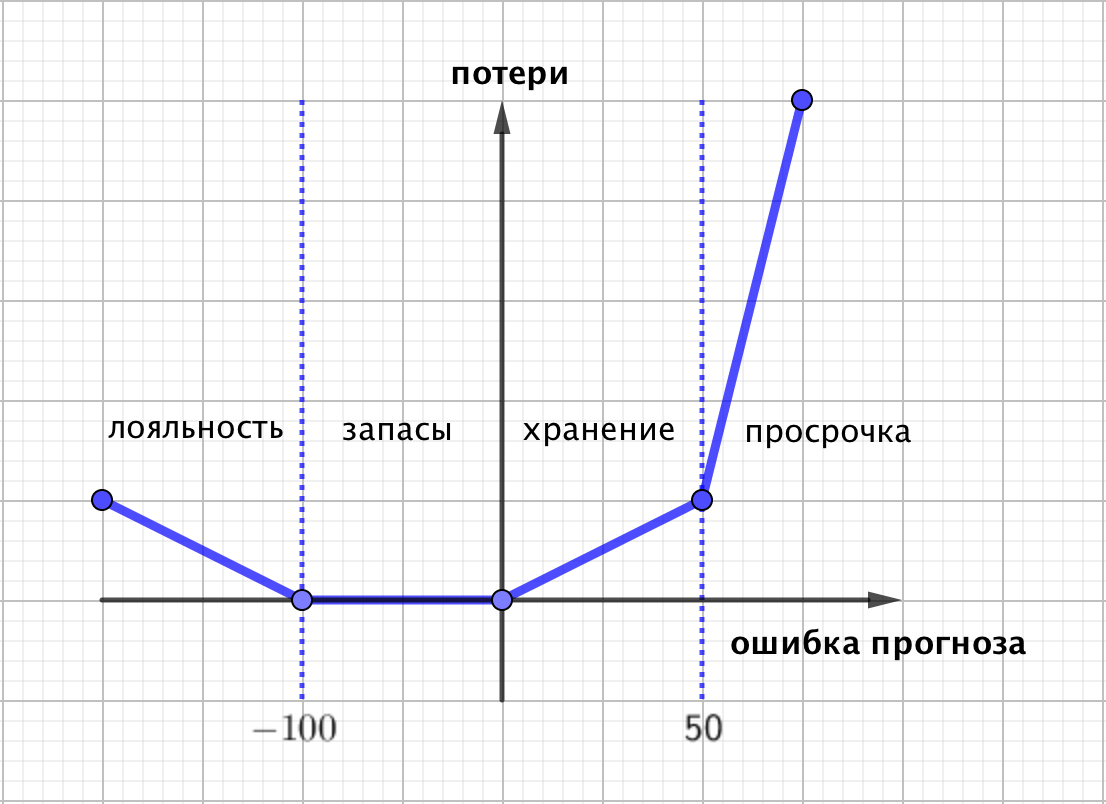
\includegraphics[scale=0.2]{err_kusok.png}
\end{center} 	

Если мы спрогнозировали слишком маленький спрос, мы произведём мало товара и его не хватит всем покупателям. Идём по оси $x$ налево. Поначалу наш косяк смогут закрыть резервы со склада. И мы не будем терпеть никаких убытков. Но рано или поздно они подойдут к концу. Предположим, что на складе хранится $100$ единиц товара. Тогда, если мы пробьём своей ошибкой его объём, получится не очень хорошая ситуация. 

Приходят к нам потребители и говорят: мы хотим телевизор. А у нас нет. На складе пусто. Ну потребитель и говорит нам, что пошел в другой магазин, раз у нас пусто. Мы теряем лояльность потребителя и, скорее всего, в следущий раз он пойдёт сразу в другой магазин. Это страшно. Поэтому начиная с отметки в $-100$  у нас появляется ошибка. Насколько крутой она будет, зависит от того, как быстро тает лояльность пользователя. Это нужно как-то оценивать по данным. И это отдельная задача. 

Если мы спрогнозировали слишком большой спрос, мы наклепаем лишнего товара. Движемся по оси $x$ направо. Если мы произвели не особо много лишнего, можно положить весь товар на склад до лучших времён. Мы будем нести издержки на хранение. У кривой потерь будет один угол. Если товара было произведено слишком много, часть просрочится. Там мы должны будем выкидывать на помойку и угол у потерь будет более крутым. Например, на картинке, мы нарисовали потери так, что если перепрогноз был больше, чем на $50$ единиц, то будет просрочка. Откуда взять это число? Опять же надо посмотреть на реальные данные и понять начиная с какой отметки товар точно будет портится. 

Для кусочно-линейной функции потерь можно придумать довольно большое количество разных ситуаций и углов в зависимости от безнесовой составляющей вашей задачки. 

\item \textbf{MSE (mean squared error), средняя квадратичная ошибка.} 

Все три метрики, о которых мы уже поговорили, линейно накидывают потери за ошибку. А, что если мы хотим более большие потери штрафовать более сильно, при этом ещё и нелинейно? Тут нам на помощь приходит штука по названием \textbf{средняя квадратичная ошибка.} Считается по формуле 

$$ MSE = \frac{1}{n}\sum_{i=1}^{n} (y_i - \hat{y}_i)^2.$$

Для нашей ситуации она составит 

$$
MSE = \frac{1}{3} \cdot(  (5-4)^2 + (10 - 20)^2 + (100 - 110)^2) = 67
$$ 

Посчитали, на формулу посмотрели. Теперь давайте разбираться какой в этом смысл. Смысл в том, чтобы штрафовать за большие ошибки сильнее, чем за маленькие. Если мы ошиблись на 5 лайков, то в потери войдёт 25. Если мы ошиблись на 10 лайков, то в потери войдёт 100. Чем выше ошибка, тем сильнее потери. 

Вы можете сказать мне:  <<А зачем? Квантильная ошибка делает то же самое!>> Не совсем. В примере, на который мы смотрели выше, мы каждый раз умножали квантильную ошибку на одно и то же число, $2$. То есть за ошибку в $5$ лайков мы бы понесли потери размером $10$.  За ошибку в $10$ лайков мы бы понесли потери размером $20$. То есть в два раза больше. В случае MSE потери получились $25$ и $100$. То есть в $4$ раза больше. 

В квантильной ошибке пропорция между потерями всегда одинаковая, а в квадратичной ошибке она постоянно увеличивается.  Давайте нарисуем на картинке. 

\begin{center}
	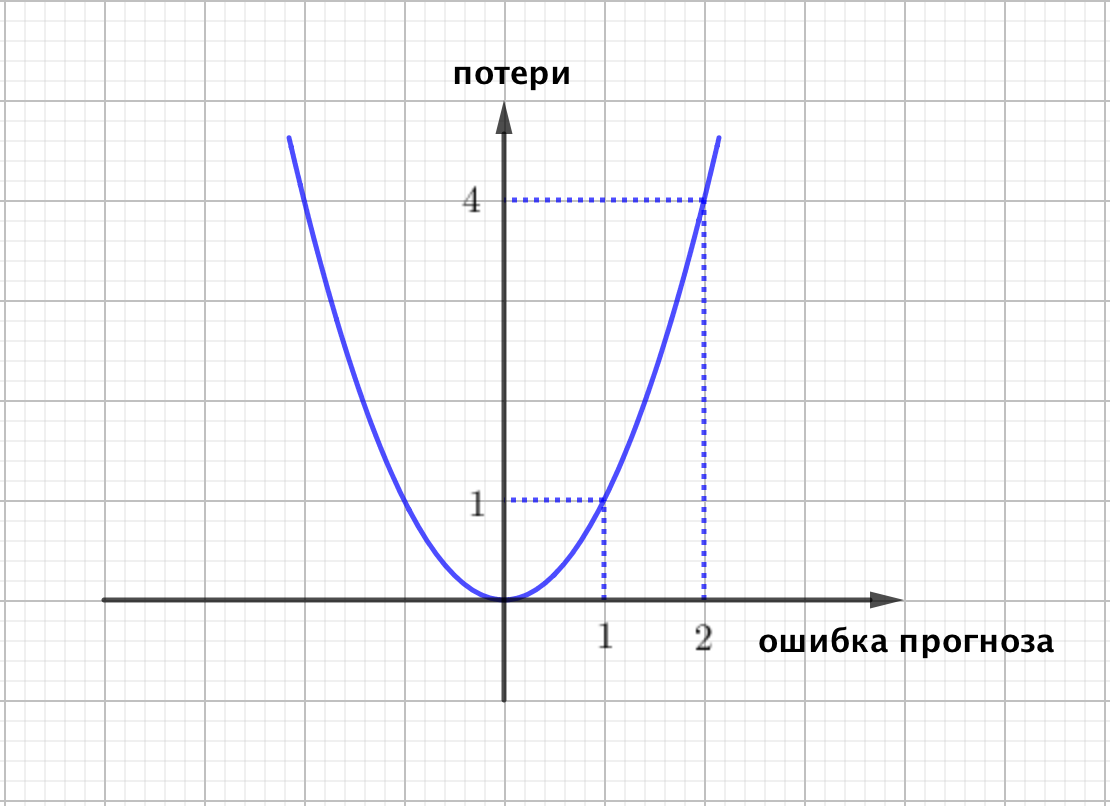
\includegraphics[scale=0.2]{err_mse.png}
\end{center} 	

Ошиблись на один лайк? Потери $1$. На два лайка? Потери $4$. На три лайка? Потери $9$. Потери каждый раз всё больше. Такова природа этой ошибки.  Из-за этого у неё возникают проблемы с выбросами. Она очень резко реагирует на них и штрафует за их наличие очень сильно.  Если вы знаете, что у вас в данных выбросы и хотите использовать $MSE$, от них нужно избавиться. 

Вопрос: а чувствительна ли к выбросам  $MAE$? Ответ: нет, потому что там идёт сумма по модулю и нет более жёсткого штрафа за более высокие отклонения.

\item \textbf{RMSE (root mean squared error)} 

Когда мы говорили про MAE, мы выяснили, что потери в её случае измеряются в лайках. Ну или в телевизорах. Для MSE мы каждое слагаемое возводим в квадрат и итоговая сумма измеряется в квадратных лайках или телевизорах. Ну или на худой конец в квадратных попугаях. Можно извлечь из MSE квадратный корень. Тогда получится новая ошибку, RMSE. Посчитаем её для нашей ситуации: 

$$
RMSE = \sqrt{MSE} = \sqrt{67}  \approx 8.19
$$

Из-за того, что более большие ошибки для нас страшнее, RMSE обычно получается больше, чем MAE. 

\item \textbf{MAPE (mean absolute percentage error)} 

Последний герой нашей задачки про метрики. Часто для нас принципиальным является не то, на сколько лайков мы ошиблись, а то на сколько процентов мы ошиблись. Метрика, которая отлавливает процентную ошибку, называется MAPE (mean absolute percentage error), средняя абсолютная процентная ошибка. 

$$
MAPE = \frac{1}{n} \sum_{i=1}^n \frac{|y_i - \hat{y}_i|}{y_i}
$$

Если вы предсказали  $1$, а в реальности было  $10$ --- это не то же самое, что вы предсказали  $1000$, а в реальности было $1009$. С точки зрения МАЕ или MSE, это две совершенно одинаковые ошибки. А если вас интересует, в среднем на сколько процентов вы ошибаетесь, то это отражает МАРЕ.  В первой ситуации мы ошиблись на $100 \cdot \frac{|1 - 10|}{10} = 90$ процентов реального результата. Во второй ситуации на $100 \cdot \frac{|1000 - 1010|}{1009} \approx 1$ процент реального результата.  Часто MAPE используют в финансах.  Давайте посчитаем метрику для нашей выборки.

$$
MAPE = 100\cdot \frac{1}{3} \cdot\left( \frac{|5 - 4|}{5} + \frac{|10 -20|}{10} + \frac{|100 - 110|}{100} \right) =  43 \% 
$$

В среднем при каждом прогнозе мы ошибаемся на $43\%$ от реального результата. 
	
\end{itemize} 
}


\subsection*{Задача 3 (как выглядит модель)}

Предположим, Олег хочет купить автомобиль и считает сколько денег ему нужно для этого накопить\footnote{сделано по мотивам \url{https://vas3k.ru/blog/machine_learning/}}. Он пересмотрел десяток объявлений в интернете и увидел, что новые автомобили стоят около $20 000$, годовалые — примерно $19 000$, двухлетние — $18 000$ и так далее.

В уме Олег-аналитик выводит формулу: адекватная цена автомобиля начинается от $20 000$ и падает на $1000$ каждый год, пока не упрётся в $10 000$. Олег сделал то, что в машинном обучении называют регрессией — предсказал цену по известным данным. Давайте попробуем повторить подвиг Олега.

\begin{enumerate}
	\item[а)] Как выглядит формула в случае Олега?
	\item[б)] За сколько продать старый афон? Придумайте формулу для предсказания. Проинтерпретируйте каждый коэффициент в ней. 
	\item[в)] Сколько одежды брать с собой в путешествие?  Придумайте формулу для предсказания. Проинтерпретируйте каждый коэффициент в ней. 
	\item[г)] Сколько шашлыка брать на дачу? Как выглядит формула?
	\item[д)] Сколько брать шашлыка, если есть толстый друг? Как можно назвать толстого друга в терминах машинного обучения? Испортит ли толстый друг формулу?
\end{enumerate}

Было бы удобно иметь формулу под каждую проблему на свете. Но взять те же цены на автомобили: кроме пробега есть десятки комплектаций, разное техническое состояние, сезонность спроса и еще столько неочевидных факторов, которые Олег, даже при всём желании, не учел бы в голове. Люди тупы и ленивы — надо заставить вкалывать роботов.

\ifbool{answers}{
	\textbf{Решение:}
	
	\begin{enumerate}
		\item[а)]  Формула Олега: $y_i = 20000 - 1000 \cdot x_i$, где $y_i$--- цена машины, $x_i$ --- её возраст. Если бы мы собрали данные о машинах и загнали их в компьютер, нам нужно было бы оценить модель
		
		\[ y_i = \beta_0 + \beta_1 \cdot  x_i.\]
		
		Коэффициент $\beta_0$ отражает базовую стоимость машины, а $\beta_1$ то, насколько она дешевеет с каждым годом. 
		
		\item[б)]  Я не знаю, к чему мы пришли при обсуждении на семинаре, но скорее всего к чему-то похожему на случай Олега. 
		
		\item[в)]  Это зависит как минимум от двух вещей: длительности поездки и пола. Девушкам обычно нужно больше вещей. Формула для обучения может выглядеть, например, вот так: 
		
		\[ 
		y_i = \beta_0 + \beta_1 \cdot  x_i + \beta_2 \cdot femail_i \cdot x_i,
		\]
		
		где $x_i$ --- срок поездки, а $femail_i$ принимает значение $1$, если путешественник --- девушка. Тогда коэффициент $\beta_1$ будет говорить сколько дополнительной одежды нам надо взять, если срок путешествия увеличивается на один день. Коэффициент $\beta_2$ будет говорить на сколько единиц одежды надо взять больше, на каждый дополнительный день, если путешественник --- девушка. Коэффициент $\beta_0$ --- какое-то базовое количество одежды, которое надо взять с собой в любом случае. 
		
		\item[в)]   Это зависит от числа людей и числа дней, на которое мы едем на дачу. Наверное логично было бы брать полкило на человека в день, то есть $y_i = 0.5 \cdot x_i \cdot z_i$, где $x_i$ --- число человек, $z_i$ --- число дней. Модель получилась нелинейной. 
		
		Можно линеаризовать её. Обычно это делается с помощью логарифмирования: 
		
		\[ \ln y_i = \ln 0.5 + \ln x_i + \ln z_i.\]
		
		В данном случае мы подобрали все коэффициенты из головы, задействовав свой природный оцениватель. Другой путь: собрать данные о поездках на дачу и заставить компьютер оценить модель: 
		
		\[ \ln y_i = \beta_0 + \beta_1 \cdot \ln x_i + \beta_2 \cdot \ln z_i.\]
		
		Такие модели, записанные в логарифмах интерпретируются чуть сложнее линейных. Коэффициент $\beta_1$ отражает то, на сколько процентов будет расти количество необходимого шашлыка, при росте числа людей на $1\%$. Коэффициент $\beta_2$ будет говорить, на сколько процентов будет расти количество необходимого шашлыка, при увеличении числа дней.
		
		\item[г)]   Если есть толстый друг, он много ест. Это выброс. Если использовать модель выше для этого друга, то нам не хватит еды. Он всё съест. Если оценивать модель по выборке, включающей толстого друга, то она подстроится под него и будет выдавать плохие прогнозы для обычных людей. 
		
		Можно модернизировать нашу модель и ввести на этого друга дамми-переменную, которая будет принимать значение $1$, если наблюдение --- он, и $0$, если кто-то другой. Модель тогда будет выглядеть: 
		
		\[ \ln y_i = \beta_0 + \beta_1 \cdot \ln x_i + \beta_2 \cdot \ln z_i + \beta_3 \cdot fat_i.\]
		
		Тогда после оценивания модели коэффициент $\beta_3$ будет отражать то, сколько шашлыка надо взять чисто для толстого друга. 
		

	\end{enumerate}	
	
	\textbf{Очень важно} понимать, что интерпретация коэффициентов верна только в тех случаях, когда мы изменяем только одну какую-то переменную. Более того, все эти изменения верны в среднем, а не для каждого конкретного случая. То есть в модели 
	
	\[ y_i = \beta_1 \cdot  x_i + \beta_2 \cdot  z_i \]
	
	значение $y$ в среднем (не всегда) увеличится на $\beta_1$, при увеличении $x_i$ на $1$, если при этом $z_i$ останется неизменной (при прочих равных).
}


\subsection*{Задача 4  (как обучаются модели)}

Давайте попробуем совсем-совсем на пальцах почувствовать как модели обучаются. Пусть у Хозяина мемов есть две переменные: $x$ --- возраст подписчика, $y$ --- число лайков, которое он оставил. Хозяин мемов хочет оценить регрессию $y = \beta \cdot x$, то есть он хочет попытаться предсказать число лайков по возрасту подписчика. Хозяин собрал два наблюдения для оценивания модели: $x_1 = 15, y_1 = 10$ и $x_2 = 22, y_2 = 2$.

Теперь хозяину надо подобрать коэффициент $\beta$ так, чтобы ошибка прогноза, измеряемая с помощью $MSE$ оказалась поменьше. 

\begin{enumerate} 
	\item  Пусть $\beta = 1$. Какие значения нам спрогнозирует модель? Какая у неё будет ошибка? 
	
	\item Пусть $\beta = 0.5$. Найдите прогнозы и ошибку модели. 
	
	\item  Какое значение для $\beta$ нам больше подходит? Как можно найти оптимальное $\beta$? 
\end{enumerate}  

\ifbool{answers}{
	\textbf{Решение:}
	
	При $\beta = 1$ получаем прогнозы $\hat y_1 = 1 \cdot 15 = 15  \hat y_2 = 1 \cdot 22 = 22$. Находим ошибку: $MSE = (15 - 10)^2 + (22 - 2)^2 = 25 + 400 = 425$. 
	
	При $\beta = 0.5$ получаем прогнозы $\hat y_1 = 5$ и $\hat y_2 = 7.5$. Ошибка составит $MSE = (10 - 5)^2 + (7.5 -2)^2 = 25 + 30.25 = 55.25$. 
	
	В случае $\beta = 0.5$ ошибка ниже. Методом перебора мы можем найти оптимальное значение $\beta$ для нашей формулы. Конечно же на практике компьютеры не перебирают влоб все возможные значения. Они делают перебор по-умному. Обычно находят производную функции ошибки по параметру $\beta$ и по ней понимают куда надо шагать и какое значение $\beta$ надо проверить на "оптимальность" следующим. Такой перебор называется градиентным спуском.  Но о нём мы поговорим подробнее как-нибудь в другой раз.  {\color{red}  \textbf{ЭТОТ ДЕНЬ НАСТАЛ!} }
}

\section*{Ещё задачи} 

Тут находится несколько задачек, о которых вам нужно подумать самостоятельно. Возможно, что похожие задачи попадутся вам на самостоятельной работе.


\subsection*{Задача 5 (картинки)}

Вот несколько ситуаций, как на ваш взгляд должны пройти линии регрессии? Да, это тоже машинное обучение. Но обычно кривые рисуем не мы, а комплюхтер.

\begin{minipage}[t]{0.45\textwidth}
	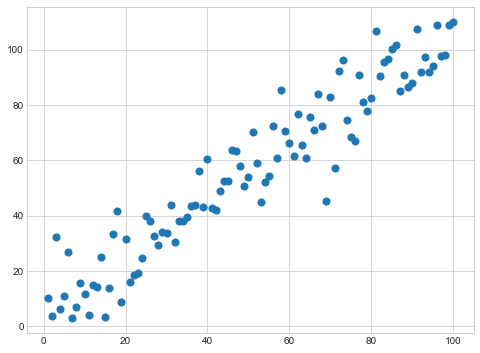
\includegraphics[scale=0.38]{regr_pic_1.png}
\end{minipage}
\hfill
\begin{minipage}[t]{0.45\textwidth}
	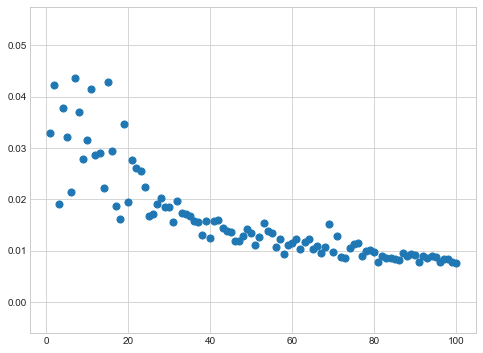
\includegraphics[scale=0.38]{regr_pic_2.png}
\end{minipage}

\begin{minipage}[t]{0.45\textwidth}
	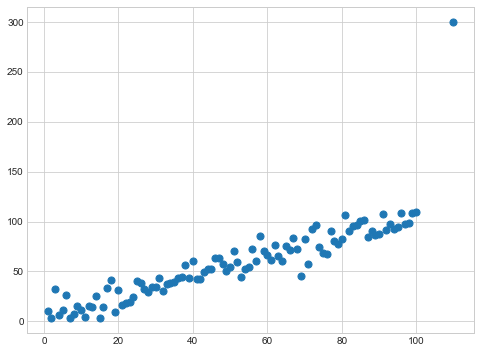
\includegraphics[scale=0.38]{regr_pic_3.png}
\end{minipage}
\hfill
\begin{minipage}[t]{0.45\textwidth}
	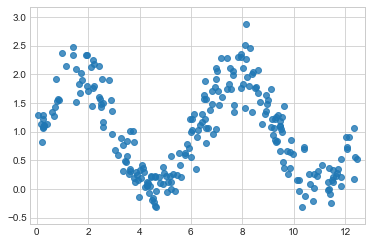
\includegraphics[scale=0.5]{regr_pic_4.png}
\end{minipage}

\begin{enumerate}	
	\item[а)] Нарисуйте на каждой из картинок линию регрессии.
	\item[б)] Как выглядят уравнения регрессии в этих ситуациях? Какие параметры в них нам нужно обучить?
	\item[в)] В чём проблема на картинке слева снизу? Проинтерпретируйте её на примере шашлыков.
	\item[г)] В четвёртой ситуации мы выбрали для обучения полином. А почему бы не взять его в каждой ситуации и не обучить через каждую точку? 
	\item[д)] Ещё одна, на этот раз трёхмерная картинка! Слабо дополнить её также, как мы делали это выше? Как будет выглядеть уравнение регрессии?
\end{enumerate}

\begin{center}
	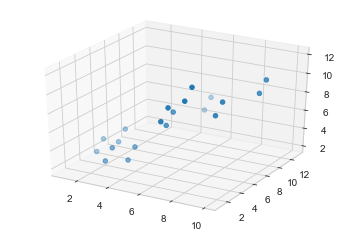
\includegraphics[scale=0.8]{regr_pic_5.png}
\end{center}


\ifbool{answers}{
	\textbf{Решение:}
	
	
	\begin{enumerate}	
		\item[а)] Берём и рисуем! 
		
		\begin{minipage}[t]{0.45\textwidth}
			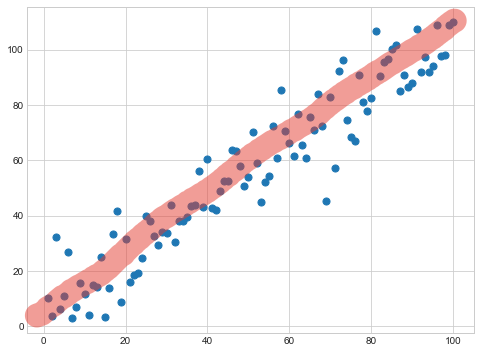
\includegraphics[scale=0.4]{regr_pic_1_ans.png}
		\end{minipage}
		\hfill
		\begin{minipage}[t]{0.45\textwidth}
			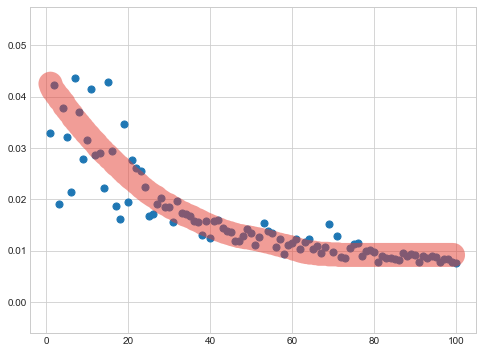
\includegraphics[scale=0.4]{regr_pic_2_ans.png}
		\end{minipage}
		
		\begin{minipage}[t]{0.45\textwidth}
			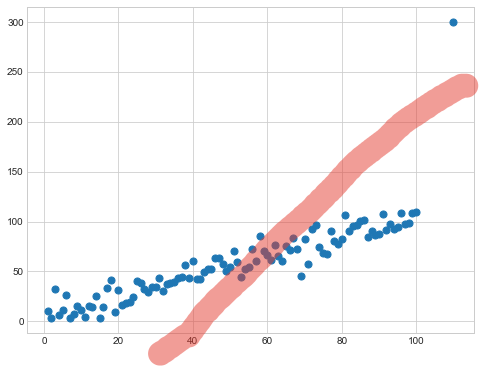
\includegraphics[scale=0.4]{regr_pic_3_ans.png}
		\end{minipage}
		\hfill
		\begin{minipage}[t]{0.45\textwidth}
			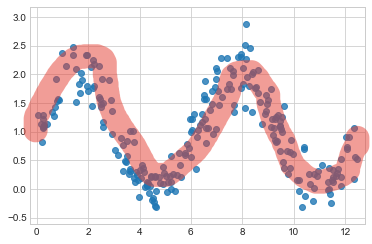
\includegraphics[scale=0.55]{regr_pic_4_ans.png}
		\end{minipage}
		
		
		\item[б)]  В первой ситуации это обычная линейная модель $y_i = \beta_0 + \beta_1 x_i$. Во второй ситуации перед  нами нелинейная модель. Внешне картинка похожа на гиперболу. Можно попробовать обучить модель $y_i = \frac{1}{\beta_0 + \beta_1 x_i}$. Однако на практике обычно поступают иначе. Если взять от $x_i$ логарифм, то модель стане линейной, и модно будет обучить $y_i = \beta_0 + \beta_1 \ln x_i$. В третьей ситуации это снова обычная линейная модель. В четвёртой ситуации это либо многочлен, либо какой-нибудь косинус. Об этих двух ситуациях мы поговорим подробнее ниже. 
		
		\item[в)]  Это толстый друг, который много ест.  Он портит обучение модели и прямая, вместо того, чтобы пройти через облако точек, подстраивается под него. Такие ситуации обычно называют выбросами. Если последовать рецепту из первого упражнения и наложить на тостого друга дамми, то ситуация нормализируется, и красная прямая пройдёт сквозь облако также как и в первой ситуации. Это эквивалентно тому, что мы выбрасываем друга из выборки и работаем с ним отдельно.
		
		Другой путь: использовать модели, которые нечувствительны к выбросам. Внимательный студент помнит как мы обсуждали на семинаре по статистике то, что медиана нечувствительна к выбросам. Можно попробовать 
		
		\item[г)]  В четвёртой ситуации мы взяли полином. Возможно, у вас возник соблазн обучить и в первых трёх ситуациях модель, которая пройдёт через все возможные точки. Это неправильно. В таком случае наша модель слишком сильно вылизывает данные. Обычно в них много шума, и модель подстраивается под него, вместо того, чтобы вычленить сигнал. Это обычно называют переобучением.
		
		\item[д)]  В этой ситуации мы строим модель не на одну переменную ($y$ на $x$), а на две ($y$ на $x$ и на $z$). Уравнение будет иметь вид $y_i = \beta_0 + \beta_1 \cdot x_i + \beta_2 \cdot z_i$. В алгебре такое уравнение описывает двумерную плоскость в трёхмерном пространстве. Новость: в трёхмерном случае мы учим не линию, а плоскость. Если размерность пространства ещё больше, мы учим некоторую гиперплоскость. 
		
		\begin{center}
			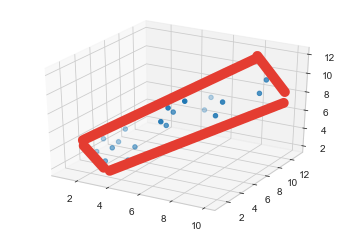
\includegraphics[scale=0.8]{regr_pic_5_ans.png}
		\end{center}
		
	\end{enumerate}
}


\subsection*{Задача 6 }

Драгомир пытается предсказать продажи видео-игр.  Для моделирования он использует две переменные: $x_1$ --- возраст игры, $x_2$ --- на кого она ориентирована. Если на мужчин, $x_2=1$, если на женщин, $x_2=0$. Целевая переменная $y$ --- сумма продаж. Драгомир оценил линейную регрессию: 

$$ y = 1000 - 100 \cdot  x_1 + 200 \cdot  x_2.$$

Проинтерпретируйте полученные коэффициенты.  Предположим, что мы выпускаем на рынок свежую игру для женщин. Спрогнозируйте наши продажи. 

%\ifbool{answers}{
%	\textbf{Решение:}
%
%Получается, что $\beta_0 = 1000$ --- это базовые продажи, $\beta_1 = -100$ --- насколько падают продажи с каждым новым годом её присутсвия на рынке, $\beta_2 = 200$, насколько выше продажи игр, которые ориентированны на мужчин.
%
%Чтобы сделать прогноз, просто подставим в уравнение интересующие нас условия: 
%
%\[ 
%y_{new} = 1000 - 100 \cdot 0 + 200 \cdot 0 = 1000
%\]
%
%}

\subsection*{Задача  7}

Маше $13$ лет. Всю свою жизнь она занималась коллекционированием моделей.  Вчера она пообщалась с Мишей. Он тоже коллекционер. Он спросил у неё, какое у её моделей качество? Маша не смогла ответить и решила проверить его. У неё есть три наблюдения $y_i$. Она для каждого построила прогнозы. Найдите для её прогнозов $MAE$, $MSE$, $RMSE$ и $MAPE$.  В чём измеряются эти ошибки? Проинтерпретируйте их. 

\begin{center}
	\begin{tabular}{c|c|c|c}
		$y_i$ &  1 & 2 & 3 \\
		\hline
		Нейросеть & 2 & 3 & 1  \\
		Регрессия &  2 & 3 & 4 \\
		Случайный лес & 1 & 1 & 1 \\
	\end{tabular}
\end{center}



\subsection*{Задача 8}

Объясните мемас: 

\begin{center}
	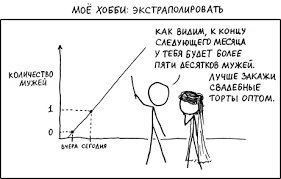
\includegraphics[scale=0.7]{memes.png}
\end{center}


\subsection*{Задача 9}

В какой	из следующих ситуаций какую метрику качества вы бы использовали?  Почему? Постарайтесь обосновать свой выбор с точки зрения бизнеса. Для удобства будем в каждом пункте обозначать наблюдаемый спрос/цену/вес и тп как  $y_i$, а наши прогнозы как  $\hat y_i$.

\begin{itemize} 
	\item Марк и Семён решили накачаться. У них есть модель, которая прогнозирует их набор массы в зависимости от рациона. По вердиктам этой модели парни заказывают себе еду на неделю. В конце недели они взвешиваются и смотрят насколько сильно модель ошиблась.
	
	\item Коста собирается устроить вечеринку. Для неё ему понадобится шашлык  (внезапно). Есть прогнозная модель, которая позволяет прикинуть сколько шашлыка ему понадобится. Он построил прогнозы для прошлой вечеринки и задумался о том какую метрику нужно выбрать для оценки качества её работы. На прошлой тусе ели только шашлык. На этой тусе, кроме шашлыка будет ещё и пицца.  Предположим, что у Косты есть один толстый друг. Возможно, он будет есть шашлык, но вот вообще не факт. 
		
	\item  Кот Матроскин продаёт молоко. Каждую неделю он прогнозирует спрос на молоко и поставляет его в торговые точки в соответствии с прогнозами. Каждая бутылка продаётся за $40$ рублей. Если он завозит слишком много, молоко портится и Матроскин теряет деньги, потраченные на производство молока и различные логистические издержки (перевозка и т.п.). Потери составляют $60$ рублей с каждой просроченной бутылки. 
	
	\item Мистер Белфорд торгует на бирже. Каждую неделю он отсчитывается перед инвесторами, рассказывая сколько дополнительных процентов от стартовых инвестиций принёс его алгоритм торговли. Внутрь алгоритма вшита прогнозная модель. Как лучше всего мистер Белфорд мог бы оценить её качество? 
\end{itemize} 

\end{document}
